\setauthor{Martin Hausleitner}
\section{Technologieevaluierung}

Ein zentraler Aspekt jedes Projektbeginns ist die Evaluierung der Technologie. Wir haben uns bewusst viel Zeit genommen, um eine schnelle und unkomplizierte Entwicklung zu ermöglichen und später mögliche Bedauern zu vermeiden. Die Anforderungen für das Projekt umfassen:

\begin{itemize}
    \item Entwicklung von Apps für Android und iOS
    \item Möglichkeit zur zukünftigen Veröffentlichung der Anwendung als Webapp
    \item Unterstützung von Datenbankabfragen auf Grundlage von Geo-Koordinaten
    \item Integrierte Authentifizierungs- und Autorisierungsschicht
    \item Realtime-Datenbank, um Echtzeit-Chatrooms für Konversationen zu führen.
\end{itemize}

\subsection{Frontend}

Im Bereich der Frontend-App-Entwicklung stehen verschiedene Möglichkeiten zur Verfügung, um eine App zu programmieren:
\begin{itemize}
    \item Native Entwicklung für jede Plattform (iOS, Android, Web)
    \item Nutzung eines Frameworks für plattformübergreifende Entwicklung von Apps
\end{itemize}

Native Entwicklung für jede Plattform (iOS, Android, Web):
Die native Entwicklung ist eine Möglichkeit, eine App speziell für eine bestimmte Plattform wie iOS, Android oder das Web zu entwickeln. Hierbei wird die App in der nativen Sprache der Plattform programmiert, d.h. in Swift für iOS, Java oder Kotlin für Android und HTML, CSS und JavaScript für das Web. Der Vorteil der nativen Entwicklung besteht darin, dass die App die native Funktionalität des Geräts vollständig nutzen und eine optimale Performance bieten kann. Entwickler können auf alle nativen APIs zugreifen und die Benutzeroberfläche der App kann besser an das jeweilige Betriebssystem angepasst werden. Allerdings erfordert die native Entwicklung spezialisierte Kenntnisse in den verschiedenen Plattformen und Programmiersprachen. Dies bedeutet, dass mehrere Entwickler benötigt werden und die Entwicklung teurer und zeitaufwändiger sein kann.

Ein Framework für plattformübergreifende Entwicklung ermöglicht die Erstellung einer einzigen Codebasis, die auf verschiedenen Plattformen wie iOS, Android und dem Web ausgeführt werden kann. Ein solches Framework nutzt häufig eine gemeinsame Programmiersprache wie JavaScript und bietet eine Vielzahl von Bibliotheken und Tools, um die Entwicklung zu erleichtern. Das Framework ermöglicht es Entwicklern, schnell und effizient Apps zu erstellen, ohne sich mit den Unterschieden in den Plattformen und Programmiersprachen auseinandersetzen zu müssen. Ein weiterer Vorteil von Frameworks für plattformübergreifende Entwicklung besteht darin, dass sie eine schnellere Markteinführung ermöglichen und den Entwicklungsaufwand reduzieren können. Allerdings kann die Verwendung eines Frameworks die Performance beeinträchtigen, da es schwierig sein kann, die App für jede Plattform zu optimieren.

Wir haben schnell beschlossen, dass wir diese Sache nicht mit nativer Programmierung angehen werden. Keiner in unserem Team ist mit einer der Plattformen vertraut, was zu einem doppelten Arbeitsaufwand führen würde. Für ein kleines Team von nur drei Personen wäre dies zeitlich einfach zu aufwendig.

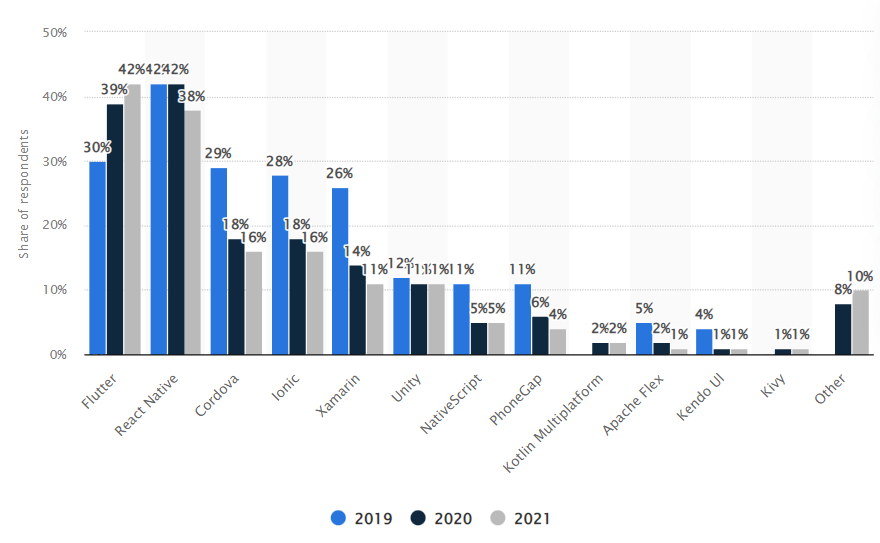
\includegraphics[width=1\textwidth]{pics/cross-platform-statisitics.png}

https://www.statista.com/statistics/869224/worldwide-software-developer-working-hours/

Um eine effektive und plattformübergreifende Entwicklung zu gewährleisten, haben wir uns dazu entschieden, ein Cross-Platform-Framework zu verwenden. Wir haben die Statistik darüber betrachtet, welche Plattformen am meisten genutzt werden und dabei festgestellt, dass Flutter mit 42 Prozent das meistgenutzte Framework ist und die Tendenz steigend ist. Auf Platz 2 liegt React Native, das fast genauso beliebt ist.

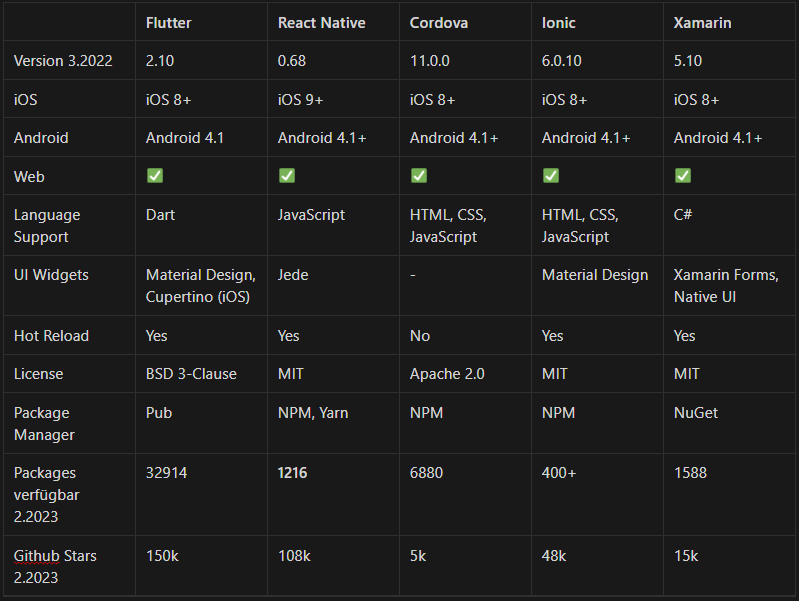
\includegraphics[width=1\textwidth]{pics/temp-table.png}

% |  | Flutter | React Native | Cordova | Ionic | Xamarin |
% | --- | --- | --- | --- | --- | --- |
% | Version 3.2022 | 2.10 | 0.68 | 11.0.0 | 6.0.10 | 5.10 |
% | iOS | iOS 8+ | iOS 9+ | iOS 8+ | iOS 8+ | iOS 8+ |
% | Android | Android 4.1 | Android 4.1+ | Android 4.1+ | Android 4.1+ | Android 4.1+ |
% | Web | Ja | Ja | Ja | Ja | Ja |
% | Language Support | Dart | JavaScript | HTML, CSS, JavaScript | HTML, CSS, JavaScript | C Sharp |
% | UI Widgets | Material Design, Cupertino (iOS) | Jede | - | Material Design | Xamarin Forms, Native UI |
% | Hot Reload | Yes | Yes | No | Yes | Yes |
% | License | BSD 3-Clause | MIT | Apache 2.0 | MIT | MIT |
% | Package Manager | Pub | NPM, Yarn | NPM | NPM | NuGet |
% | Packages verfügbar 2.2023 | 32914 | 1216 | 6880 | 400+ | 1588 |
% | Github Stars 2.2023 | 150k | 108k | 5k | 48k | 15k |

Quellen:
[https://reactnative.directory/](https://reactnative.directory/)

[https://pub.dev/](https://pub.dev/)
[https://www.npmjs.com/search?q=keywords:ecosystem:cordova](https://www.npmjs.com/search?q=keywords:ecosystem:cordova)
[https://github.com/xamarin](https://github.com/xamarin)
[https://github.com/apache/cordova-android](https://github.com/apache/cordova-android)

[https://ionic.io/docs/supported-plugins](https://ionic.io/docs/supported-plugins)

[https://market.ionicframework.com/plugins](https://market.ionicframework.com/plugins)

In der Vergleichstabelle haben wir die wichtigsten Informationen zu den verschiedenen Frameworks zusammengefasst. Dabei haben wir festgestellt, dass alle Plattformen unsere Anforderungen erfüllen. Xamarin hat für uns als Team, das seit Jahren C\# programmiert, ein gewisses Interesse geweckt. Allerdings hat Dart eine ähnliche Syntax wie C\#, weshalb es für uns als Team auch eine geeignete Option darstellt.

Flutter hat als UI-Widget-Library sowohl Material Design 2 und 3 als auch eine iOS Library, die das native iOS-Design 1:1 abbildet. Dadurch kann der Nutzer den Unterschied zwischen nativen und Flutter-Designs kaum erkennen. Xamarin hat ebenfalls eine UI-Library namens Xamarin.Forms, die auf allen Plattformen funktioniert und native UI-Libraries für jede Plattform enthält.

React Native ist zwar in JavaScript geschrieben, aber man kann keine React-Komponenten importieren und verwenden. Wenn man jedoch bereits Erfahrung mit React.js hat, kann man sich als Entwickler leichter in React Native einarbeiten. Die letzten beiden Plattformen Cordova und Ionic basieren auf HTML, CSS und JavaScript, was den Vorteil bietet, dass man auf jede JavaScript-Library zugreifen kann.

Ein wichtiger Faktor bei der Wahl des Frameworks ist auch der Hot Reload. Cordova bietet diese Funktion nicht, alle anderen Plattformen hingegen schon, was für uns ein dealbreaker ist.

Die Package-Manager wurden ebenfalls verglichen und der von Flutter hat uns am meisten überzeugt, da jedes Package ein Beispiel hat und man anhand von Pub Points sehen kann, wie gut das Package in verschiedenen Kriterien abschneidet. Zudem kann man sehen, welche Plattformen das Package unterstützt.

Obwohl npm der meistgenutzte Package-Manager ist, ist er nicht spezifisch auf ein bestimmtes Framework ausgerichtet und es fehlen einige Funktionen, die Pub hat. NuGet kennen wir bereits von der CSharp-Entwicklung und unserer Meinung nach wirkt er sehr altmodisch und fehlt ebenfalls einige Funktionen, die Pub hat.

Ein weiterer wichtiger Faktor bei der Wahl des Frameworks sind die verfügbaren Packages. Flutter bietet hier eine große Auswahl, wobei zu beachten ist, dass bei Frameworks, die auf JavaScript basieren, auf alle JavaScript-Libraries zugegriffen werden kann. Insgesamt sind die meisten Flutter-Packages auf mobile Apps ausgerichtet.

Die Community wurde anhand der Anzahl der Github-Stars gemessen, wobei Flutter mit gut einem Drittel vor React Native liegt. Obwohl Flutter noch nicht so lange auf dem Markt ist, spricht dies dafür, dass Entwickler mit Flutter sehr zufrieden sind.

Ein wichtiger Aspekt bei der Verwendung von Cross-Platform-Frameworks ist die Performance, da diese aufgrund ihrer Nicht-Nativität variieren kann. In einem Forschungspapier, in dem alle oben genannten Plattformen mit Ausnahme von Cordova verglichen wurden, wurde in Punkt 2.6 ein aussagekräftiger Vergleich durchgeführt. Dabei wurde festgestellt, dass Flutter hinsichtlich der Performance auf Platz 1 liegt, gefolgt von React Native auf Platz 2. Im Gegensatz dazu schneidet Xamarin bei diesem Vergleich nicht so gut ab. Die letzte Position nimmt Iconic ein, was aufgrund der Tatsache, dass es lediglich eine HTML-, CSS- und JavaScript-Seite in einem Webview anzeigt, nachvollziehbar ist. Im Vergleich zu den anderen Plattformen kann es aufgrund des Fehlens eigener Renderer nicht mithalten.

Quellen:
http://uu.diva-portal.org/smash/get/diva2:1626535/FULLTEXT01.pdf

% \usepackage{array}




% Nach ausführlicher Recherche wurden die folgenden plattformübergreifenden Frameworks in Betracht gezogen\cite{cross_platform_framework_comparison}: Flutter, React Native, Ionic und Xamarin. Jede Plattform hat ihre Vor- und Nachteile.

% Nach langer Recherche und Evaluierung aller Faktoren wurde Flutter als Plattform für das Frontend ausgewählt. Insbesondere das schnelle entwicklung und das einfache Debugging sowie die Integration in VS Code waren entscheidende Faktoren. Jeder aus unserem Team hat eine eigene Flutter Test App programmiert \cite{flutter_test_apps} um die entscheidung zu festigen.

% Insgesamt waren wir mit unserer Entscheidung, Flutter zu verwenden, sehr zufrieden. Während der Entwicklungszeit stellte sich heraus, dass die Klammerverwendung in Flutter am Anfang etwas ungewohnt war, aber dank der hervorragenden Unterstützung durch die Flutter-Community und der umfangreichen Dokumentation auf Stack Overflow konnten wir alle Herausforderungen bewältigen. Außerdem wurde die Entwicklung durch die ständigen Verbesserungen und Updates von Flutter, wie der Einführung der Impeller-Rendering-Engine, beschleunigt. \cite{flutter_impeller}

% Insgesamt war die Wahl von Flutter für das Frontend der App eine gute Entscheidung.

\subsection
{Backend}
Da ich über umfangreiches Wissen in verschiedenen Backend-Technologien verfüge, fiel uns die Entscheidung für unser Projekt etwas leichter. Wir konzentrierten uns bei der Auswahl auf "Backend-as-a-Service"-Plattformen, da sie bereits viele Funktionen implementiert haben und wir somit nicht alles neu programmieren mussten.

In Betracht kamen für unser Projekt drei Technologien: Supabase, Firebase und Appwrite. Alle drei bieten SDKs für Flutter und React Native. Darüber hinaus verfügen sie alle über eine Datenbank, die Geoqueries für das Hauptfeature des Beitragradius unterstützt, sowie Storage für Beitragsfotos und viele mehr

Supabase hot zum Zeitpunkt der Evaluierung im Februar 2022 jedoch noch keine Cloud-Functions wie Firebase und Appwrite, was es schwierig machte, eine robuste Business-Logik umzusetzen. Obwohl Supabase am 1. April 2022 experimentell Edge Functions eingeführt hat, ist dies für eine Produktions-App nicht empfehlenswert.

Daher blieben Appwrite und Firebase als die beiden besten Optionen übrig. Obwohl Appwrite nicht mit den Features von Firebase mithalten konnte, ist Appwrite 100 Prozent Open Source und Firebase Closed Source, was für Appwrite spricht. Da wir uns bei unserem Cross-Platform-Framework noch nicht sicher waren, war es uns nun leichter, uns für Firebase zu entscheiden, da es das beste Flutter-SDK hatte, was man anhand der verfügbaren Features erkennen konnte.

% Für die Implementierung einer mobilen App in Flutter für die Diplomarbeit von Martin Hausleitner wurden verschiedene Backend-Technologien evaluiert. Dabei wurden folgende Anforderungen an die Technologie gestellt: Skalierbarkeit, Realtime-Datenbank für Chat, Business-Logik für den Beitragsradius, sichere Authentifizierung und Verschlüsselung sowie eine einfache und schnelle Entwicklungsmöglichkeit.

% Die drei Favoriten für die Backend-Technologie waren Supabase \cite{supabase}, Firebase\cite{firebase} und Appwrite\cite{appwrite}. Diese wurden alle zum damaligen Zeitpunkt (Februar 2022) mit einem Flutter-SDK unterstützt.

% Technologieevaluation für eine Diplomarbeit

% Die Wahl der richtigen Technologie für eine Diplomarbeit ist von entscheidender Bedeutung für den Erfolg des Projekts. In diesem Abschnitt werden verschiedene Technologien zur Umsetzung einer Chat-App evaluiert.

% Zu den wichtigsten Anforderungen an die Technologie gehören Skalierbarkeit, Echtzeit-Datenbank für den Chat, eine robuste Business-Logik für den Beitragsradius, sichere Verschlüsselung und eine einfache Entwicklung.

% Für unser Projekt kamen drei Technologien in frage: Supabase \cite{supabase}, Firebase\cite{firebase} und Appwrite\cite{appwrite} Sie alle bieten SDKs für Flutter und verfügen über eine benutzerfreundliche Authentifizierungsschicht. Darüber hinaus verfügen sie alle über eine Datenbank, die Geoqueries für das Hauptfeature des Beitragradius unterstützt, sowie einen Speicherplatz für Beitragsfotos.

% Allerdings bietet Supabase zum Zeitpunkt der Evaluierung im Februar 2022 noch keine Cloud-Funktionen wie Firebase und Appwrite, was es schwierig macht, eine robuste Business-Logik umzusetzen. Obwohl Supabase am 1. April 2022 experimentell Edge Functions eingeführt hat, ist dies für eine Produktions-App nicht empfehlenswert.

% Daher wurden Appwrite und Firebase als die beiden besten Optionen identifiziert. Firebase bietet bessere Flutter-SDKs und verfügt über mehr Features, einschließlich der Unterstützung von Google für Flutter, weshalb wir uns schließlich für Firebase entschieden haben.

% In der folgenden Tabelle sind die Vor- und Nachteile von Appwrite und Firebase aufgeführt:










% \begin{table}[h]
%     \centering
%     \begin{tabular}{|p{4cm}|p{6cm}|p{6cm}|}
%         \hline
%                   & \textbf{Firebase}                                                                        & \textbf{Appwrite} \ \hline
%         Vorteile  & \begin{itemize}
%                         \item Gute Dokumentation
%                         \item Einfache Integration mit Flutter-SDKs
%                         \item Umfangreiche Features wie Analytics, Performance Monitoring, Cloud Messaging, etc.
%                         \item Schnelle und einfache Entwicklung
%                     \end{itemize}
%                   &
%         \begin{itemize}
%             \item Open Source
%             \item Einfache Integration mit Flutter-SDKs
%             \item Sichere Authentifizierung und Verschlüsselung
%             \item Einfache Skalierbarkeit
%             \item Bietet auch Serverless-Funktionen
%         \end{itemize} \ \hline
%         Nachteile & \begin{itemize}
%                         \item Kostenpflichtig bei Nutzung größerer Mengen an Ressourcen
%                         \item Abhängigkeit von Google
%                     \end{itemize}
%                   &
%         \begin{itemize}
%             \item Weniger umfangreiche Features als Firebase
%             \item Keine direkte Integration mit anderen Google-Tools
%         \end{itemize} \ \hline
%     \end{tabular}
%     \caption{Vor- und Nachteile von Firebase und Appwrite}
%     \label{tab:impl:backend}
% \end{table}

% Insgesamt bietet Firebase aufgrund der umfangreichen Features und der einfacheren Integration mit anderen Google-Tools Vorteile gegenüber Appwrite.


\section{Technologie entscheidung}
Die Kombination aus Flutter und Firebase hat uns am meisten überzeugt, da sie gut harmonieren. Flutter ist ein schnelles Framework mit einer breiten Palette an Erweiterungen für mobile Anwendungen und verfügt über eine starke Community. Der Trend geht in die Richtung, dass Flutter Marktführer wird, was uns ein gutes Gefühl bezüglich unserer Entscheidung gibt. Zu Beginn gab es jedoch Zweifel bei der Arbeit mit Flutter, da es aufgrund der vielen Klammern schnell unübersichtlich wurde. Dank der super VS Code-Integration mit einem Reformat-Feature, das das Klammernproblem löst, konnten wir diese Herausforderung meistern. Auch nach einem Jahr Entwicklung mit Flutter sind wir immer noch beeindruckt davon, wie einfach es ist, Features zu implementieren und wie straight-forward die Entwicklung ist. Der Syntax von Dart, der Programmiersprache hinter Flutter, ist schnell erlernbar und ermöglicht es uns, schnell viele Programmierpatterns zu beherrschen.

Firebase hat sich ebenfalls als sehr gute Entscheidung herausgestellt, da die Entwicklung schnell und einfach ist. Ein großer Vorteil ist, dass wir uns keine Sorgen um das Skalieren machen mussten. Mit den Features ist Firebase nach wie vor die Nr. 1. Allerdings gibt es zwei große Nachteile, die unsere Backend-Entscheidung aktuell ändern würden. Die Firestore-Datenbank bietet keine Suchfunktion, weshalb wir Algolia genutzt haben. Einerseits bietet Algolia viele fortgeschrittene Suchfunktionen, die andere Datenbank-Suchmaschinen nicht haben. Allerdings ist es keine perfekte Lösung. In unserer Diplomarbeit ist auch das Thema Transparenz und Open Source von großer Bedeutung. Firebase schränkt uns hierbei ein, da es Closed Source ist. Daher würden wir nach aktuellem Standpunkt Supabase nutzen, da es mittlerweile auch Cloud Functions bietet und Open Source ist. Supabase verwendet zudem PostgreSQL, das eine Suchfunktion schon integriert hat.

% Die Wahl von Flutter als Frontend-Plattform und Firebase als Backend-Plattform erwies sich als gute Entscheidung für die Anforderungen dieser Diplomarbeit. Die Einfachheit der Syntax, das schnelle Debugging und die umfangreiche Dokumentation und Unterstützung durch die Community machten Flutter zu einer einfachen und effizienten Plattform für die Entwicklung der mobilen Apps. Firebase hat eine gute Lösung für die Echtzeit-Datenbank und die Geodatenbank und eine einfache Integration mit Flutter.

% Insgesamt haben die gewählten Technologien dazu beigetragen, dass die Entwicklung der Anwendung schnell und effizient verlief und die Anforderungen der Diplomarbeit erfüllt wurden.

